\chapter{Cellular Automata}\label{ch:CA}

Cellular Automata (CA) are parallel computing models, whose evolution
is ruled by local rules. They are largely employed in Science and
Engineering for a wide range of problems, especially when classic
methods (e.g., based on differential equations) can not be conveniently
applied. In this Chapter, CA are briefly introduced, together with a
recent extension of them, known as Extended Cellular Automata (XCA),
which are widely used for the modeling of physical extended systems.


\section{Informal Definition of Cellular Automata}\label{sec:CAInformaDef}

A cellular automaton can be thought as a $d$-dimensional space, called
\emph{cellular space}, subdivided in regular cells of uniform shape
and size. Each cell embeds a \emph{finite automaton}, one of the most
simple and well known computational models, which can assume a finite
number of states. At time $t=0$, cells are in arbitrary states and the
CA evolves step by step by changing the states of the cells at
discrete time steps, by applying the same local rule of evolution,
i.e. the cell's \emph{transition function}, simultaneously (i.e. in
parallel) to each cell of the CA. Input for the cell is given by the
states of a predefined (usually small) set of neighboring cells, which
is assumed invariant in space and time. It is possible to identify an
informal definition of cellular automaton by simply listing its main
properties:

\begin{itemize}
\item It is formed by a $d$-dimensional space (i.e. the \emph{cellular
  space}), partitioned into cells of uniform shape and size
  (e.g. triangles, squares, hexagons, cubes, etc. - see Figure
  \ref{fig:cellularspaces});
\item The number of cell's states is finite;
\item The evolution occurs through discrete steps;
\item Each cell changes state simultaneously to each other (i.e. they
  change state concurrently, in parallel) thanks to the application of
  the cell's \emph{transition function};
\item The cell's state transition depends on the states of a set of neighboring cells;
\item The evolving cell is called \emph{central cell} and can belong
  to its neighborhood;
\item The neighboring relationship is local, uniform and invariant
  over time (see Figures \ref{fig:1Dneighborhood},
  \ref{fig:2Dneighborhood}, and \ref{fig:3Dneighborhood} for examples
  of 1D, 2D, and 3D neighborhoods, respectively).
\end{itemize}

\begin{figure}
  \begin{center}
    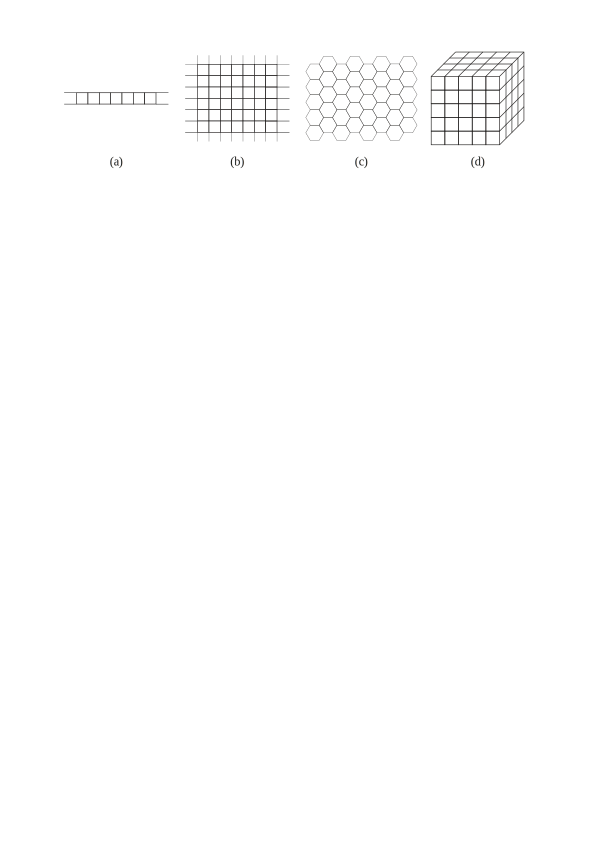
\includegraphics[width=11.5cm]{./images/CellularAutomata/cellularspaces.pdf}
    \caption{Example of cellular spaces: (a) one-dimensional, (b)
      two-dimensional with square cells, (c) two-dimensional with
      hexagonal cells, (d) three-dimensional with cubic cells.}
    \label{fig:cellularspaces}
  \end{center}
\end{figure}

\begin{figure}
  \begin{center}
    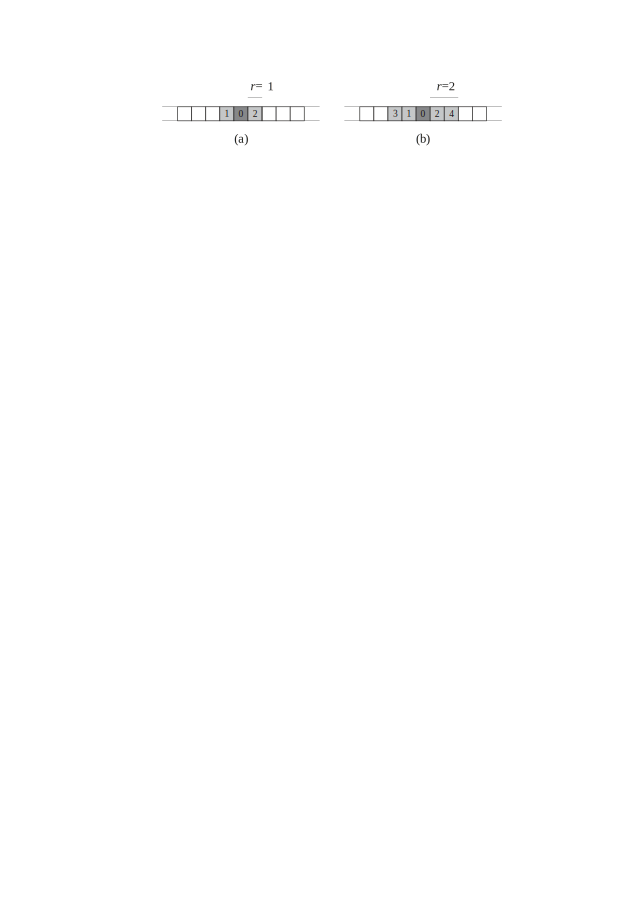
\includegraphics[width=8cm]{./images/CellularAutomata/1Dneighborhoods.pdf}
    \caption{Example of neighborhood with radius (a) $r = 1$ and (b) $r
      = 2$ for one-dimensional Cellular Automata. Central cell is
      represented in dark gray, while adjacent cells are in light
      gray. Note that the central cell can optionally belong to its own
      neighborhood.}
    \label{fig:1Dneighborhood}
  \end{center}
\end{figure}

\begin{figure}
  \begin{center}
    \includegraphics[width=11.5cm]{./images/CellularAutomata/2Dneighborhoods.pdf}
    \caption{Examples of von Neumann (a) and Moore (b) neighborhoods
      for two-dimensional CA with square cells. Examples of Moore
      neighborhoods are also shown for hexagonal CA, both for the
      cases of horizontal (c) and vertical (d) orientations. Central
      cell is represented in dark gray, while adjacent cells are in
      light gray. A reference system is here considered to evaluate
      cells coordinates in terms of row and column indices in a
      matrix-style representation, and a 0-based numerical identifier
      assigned to each cell in the neighborhood for direct
      access.}
    \label{fig:2Dneighborhood}
  \end{center}
\end{figure}

\begin{figure}
  \begin{center}
    \includegraphics[width=11.5cm]{./images/CellularAutomata/3Dneighborhoods.pdf}
    \caption{Examples of von Neumann (a) and Moore (b, b')
      neighborhoods for three-dimensional CA with cubic
      cells. Central cell is represented in dark gray, while adjacent
      cells are in light gray. A reference system is here considered
      to evaluate cells coordinates in terms of row, column and slice
      indices in a matrix-style representation, and a 0-based
      numerical identifier assigned to each cell in the neighborhood
      for direct access.}
    \label{fig:3Dneighborhood}
  \end{center}
\end{figure}

Despite their simple definition, CA can exhibit very interesting
complex global behaviors. Moreover, from a computational point of
view, they are equivalent to Turing Machines. This means, in
principle, that everything that can be computed can also be by means
of a cellular automaton (Church Turing thesis). Thanks to their
\emph{computational universality}, CA gained a great consideration
among the Scientific Community and were employed for solving a great
variety of different complex problems.

\section{Formal Definition of Cellular Automata}

Cellular Automata are formally defined as a quadruple:

$$A = <R,X,Q,\sigma>$$

\noindent where:

\begin{itemize}
\item $R = \{i = (i_0,i_1,....,i_{d-1}) \; | \; i_k \in \mathbb{Z} \;\; \forall k =
  0,1,...,d-1\}$ is the set of points, with integer coordinates, which
  defines the $d$-dimensional cellular space;

\item $X = \{\xi_0,\xi_1\,...\xi_{m-1}\}$ is the finite set of $m$
  $d$-dimensional vectors
  \[ \xi_j = \{\xi_{j_0},\xi_{j_1},...\xi_{j_{d-1}}\} \]
  that define the set
  \[ N(X,i) = \{i + \xi_0,i + \xi_1,...,i + \xi_{m-1}\} \]
  of coordinates of cells belonging the the central cell's
  neighborhood (i.e. the cell with coordinates $i =
  (i_1,i_2,...i_d)$). In other words, $X$ represents the geometrical
  pattern that specifies the neighborhood relationship;

\item $Q$ is the finite set of states of the cell;

\item $\sigma : Q^m \rightarrow Q$ is the cell's transition function.

\end{itemize}


\section{Some Applications of Cellular Automata}

CA are particularly suited to model and simulate classes of
complex systems characterized by a large number of interacting
elementary components.  The assumption that if a system behavior is
complex, the model that describes it must necessarily be of the same
complexity is replaced by the idea that its behavior can be
described, at least in some cases, in very simple terms.

Among different fields, fluid-dynamics is one of most important
applications for CA and, in this research branch, many different
CA-based methods can be found in the literature to simulate fluid
flows.  For instance, Lattice Gas Automata (LGA) were introduced for
describing the motion and collision of \emph{particles} on a grid and
it was shown that such models can reproduce the main fluid dynamical
properties. The continuum limit of these models leads to the
Navier-Stokes equations. Lattice Gas models can be regarded as
microscopic models, as they describe the motion of fluid particles
which interact by scattering. An advantage of Lattice Gas models is
that the simplicity of particles, and of their interactions, allow for
the simulation of a large number of them, making it therefore possible
to observe the emergence of flow patterns. Furthermore, since they are
CA systems, it is possible to easily run simulations in parallel. A
different approach to LGA is represented by Lattice Boltzmann models
in which the state variables can take continuous values, as they are
supposed to represent the density of fluid particles, endowed with
certain properties, located in each cell (space and time are also
discrete, as in lattice gas models). Both Lattice Gas and Lattice
Boltzmann Models have been applied for the description of fluid
turbulence.

Since many complex natural phenomena evolve on very large areas, they
are therefore difficult to be modeled at a microscopic level of
description. Among these, we can find some real flow-type phenomena
like debris and lava flows, as well as floods and pyroclastic
flows. Besides rheological complex behavior, they generally evolve on
complex topographies, that can even change during the phenomenon
evolution, and are often characterized by branching and rejoining of
the flow. In order to better model such kind of phenomena, an extended
notion of Cellular Automata (Extended Cellular Automata, described in
the next Section), can represent a valid alternative to classical CA.

\section{Extended Cellular Automata}

As regards the modeling of natural complex phenomena, Prof. Gino
Mirocle Crisci and co-workers from University of Calabria (Italy)
proposed a method based on an Extended notion of Cellular Automata
(XCA), firstly applied to the simulation of basaltic lava flows in the
80's\footnote{XCA are also known as Complex Cellular Automata (CCA),
  Macroscopic Cellular Automata (MCA), and Multicomponent Cellular
  Automata (MCA)}. It was shown that the approach behind XCA can
greatly make more straightforward the modeling of some complex
systems. Compared to classical CA, XCA are different because of the
following reasons:

\begin{itemize}

\item The cell's state is decomposed in \emph{substates}, each of them
  representing the set of admissible values of a given characteristic
  assumed to be relevant for the modeled system and its evolution
  (e.g., lava temperature, lava thickness, etc, in the case of a lava
  flow model). The set of states for the cell is simply obtained as
  the Cartesian product of the considered substates.

\item As the cell's state can be decomposed in substates, also the
  transition function can be split into \emph{elementary processes},
  each of them representing a particular aspect that rules the dynamic
  of the considered phenomenon. In turn, \emph{elementary processes}
  can be split into \emph{local interactions}, which refer to rules
  that deal with interactions among substates of the cell with
  neighbor ones (e.g., mass exchange with neighbors) and
  \emph{internal transformations}, defined as the changes in the
  values of the substates due only to interactions among substates
  inside the cell (e.g. the solidification of the lava inside the cell
  due to the temperature drop).

\item A set of \emph{parameters}, commonly used to characterize the
  dynamic behaviors of the considered phenomenon, can be defined.

\item Global operations can also be allowed (e.g. to model external
  influences that can not easily be described in terms of local
  interactions, or to perform reductions over the whole, or a subset
  of, the cellular space). They are often referred as \emph{steering}
  operations.

\end{itemize}


\subsection{Formal Definition of Extended Cellular Automata}


Formally, a XCA is defined as a 7-tuple:

$$ A = <R,X,Q,P,\sigma,\Gamma,\gamma>$$

\noindent where:

\begin{itemize}

\item $R$ is the $d$-dimensional cellular space.

\item $X$ is the geometrical pattern that specifies the neighborhood
  relationship; $m = |X|$ represent the number of elements in the set
  $X$, i.e. the number of neighbors for the central cell.

\item $Q = Q_0 \times Q_1 \times....\times Q_{n-1}$ is the set of
  cell's states, expressed as Cartesian product of the $n$ considered
  \emph{substates} $Q_0 \times Q_1 \times....\times Q_{n-1}$.

\item $P = {p_0,p_1,....,p_{p-1}}$ is the set of CA
  \emph{parameters}.They can allow a fine tuning of the XCA model,
  with the purpose of reproducing different dynamical behaviors of
  the phenomenon of interest.

\item $\sigma : Q^m \rightarrow Q$ is the cell's transition function.
  It is split in $s$ \emph{elementary processes}, $\sigma_0,\sigma_1,
  ..., \sigma_{s-1}$, each one describing a particular aspect ruling
  the dynamic of the considered system.

\item $\Gamma \subseteq R$ is the region over which steering is applied.

\item $\gamma: Q^{|\Gamma|} \rightarrow Q^{|\Gamma|} \times
  \mathbb{R}$ is the (global) steering function.

\end{itemize}

In the next Chapters, some examples of XCA will be presented. Their
implementations in OpenCAL will also be described, both in serial
(Chapter \ref{ch:opencal}) and in parallel (Chapters
\ref{ch:opencal-omp} and \ref{ch:opencal-cl}).
